%!TEX root = ../thesis.tex
\begin{savequote}[90mm]
	\hl{Scrum means ``Waterfall but we don't have time for analisys''\\
	Kanban means ``Scrum, but we don't have time for Sprint planning''\\
	Agile means ``We have no process but we do use Jira extensively''
	\qauthor{@mikeveerman on Twitter}}
\end{savequote}

\chapter{Projet implementation}
	This chapter is the core of this document and describes the way that this project has been implemented according to the planning described in Chapter 2.
	It is structured in four main sections, each representing a time period:
	\begin{enumerate}
		\item Learning stage - RIVEDERE NOME
		\item Implementation
		\item Testing
		\item Feedback
	\end{enumerate}
	Since the scope of the project was to create a testing environment to show the capabilities of Jira, Athonet has bough ten user licenses for Jira Software, ten for Service Desk and ten for Confluence.
	%todo inserire riferimento
	%https://confluence.atlassian.com/cloud/compare-atlassian-cloud-vs-server-744721664.html
	All these software have three installation options:
	\begin{itemize}
		\item Cloud
		\item Server
		\item Data Center
	\end{itemize}
	Because of Athonet's policies about storing their data in the cloud, they opted for an on premise Server installation.
	This kind of installation requires a one time payment for the software while other subsequent fees will be for the support.

\section{Learning stage - CAMBIARE NOME}

	%todo aggiungere fatto che hanno scelto di prendere il hosting plan in house rispetto a server e datacenter a causa della sicurezza dei loro dati

	This phase corresponds to the first two weeks of the internship.
	As described in the work plan in this first period the main task was to understand what the tools are.
	At first I have started to search information about Jira and Confluence on Google.
	%todo aggiungere riferimento a official documentation
	The first tools I have started researching was Jira, and the official documentation is very well organized.
	\begin{figure}[H]
		\centering
		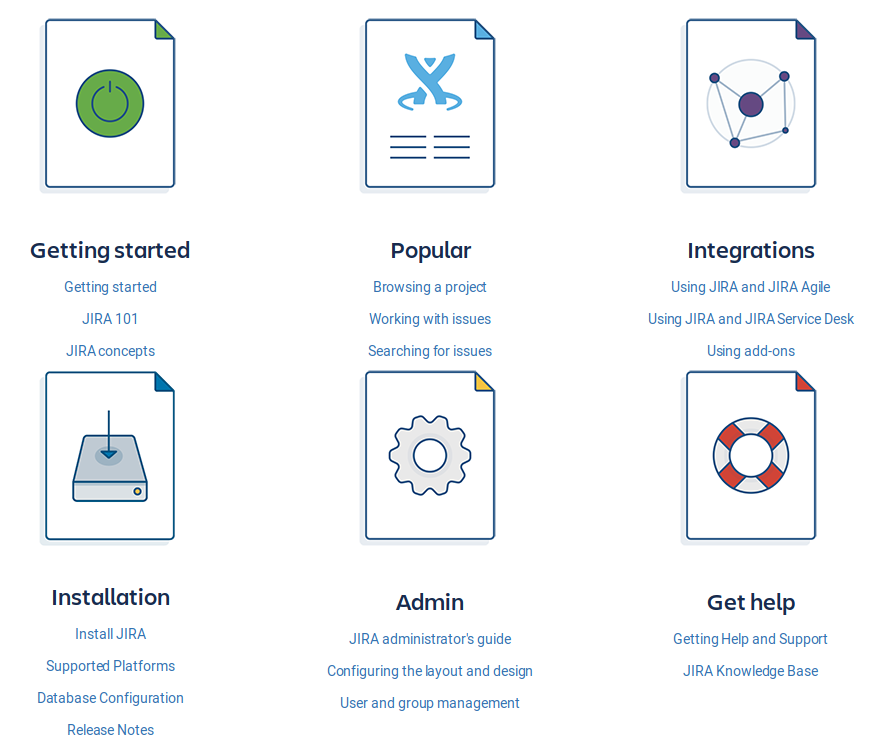
\includegraphics[width=1\textwidth]{resources/jira_documentation}\\
		\caption{Screenshot of the Jira Documentation homepage from the Atlassian Support website}
	\end{figure}
	This documentation is very easy to navigate because it versioned for each release, major and minor, of the software, plus it contains links to related pages, including Confluence's documentation and Atlassian's blog.
	%todo rivedere ripetizioni
	Same on Confluence's documentation, if there is a Jira reference, it links to the latter's documentation.	
	%todo aggiungere riferimento
	As said in ... both Jira and Confluence have a bug reporting and issue tracking section in their documentation.
	\begin{figure}[H]
		\centering
		\includegraphics[width=1\textwidth]{resources/confluence_documentation_issues}\\
		\caption{The issues related with Jira and Confluence are handled by a dedicated Jira Cloud instance}
	\end{figure}
	If a webpage in the documentation is related to an issue, the latter is showed at the end of the page with its status and a link to its dedicated section. 
	%todo rivedere parola userbase
	The Confluence and Jira documentation are both written and hosted using Confluence, showing how powerful can be this tool for handling a wiki for such a complex software that has a large userbase.
	Confluence's documentation is structured like Jira's, very easy to access and consult.	
	Another bonus is that it is public and free to consult, despite the software is not.
	This may seem like an obvious choice but not all vendors do it: RedHat for example let's you consult their documentation only if you log into the website.
	During the second half of the first week, while studying the documentation I went ahead and started configuring the environment.
	In order to install the Atlassian tools I was given a CentOS VM with 512GB of storage and 32GB of RAM, connected to a special testing environment for internship students.
	%todo aggiungere a glossario centos
	\begin{figure}[H]
		\centering
		
\includegraphics[width=1\textwidth]{resources/centos_logo}\\
		\caption{The issues related with Jira and Confluence are handled by a dedicated Jira Cloud instance}
	\end{figure}
	To connect with the remote machine I used Remmina, a remote desktop client for Linux operating systems.
	
\section{Initial installation and configuration}
	
	%todo frase introduttoria
	
	As for the previous phase, the first software I installed was Jira, by following the official documentation.
	%https://confluence.atlassian.com/adminjiraserver/installing-jira-applications-on-linux-938846841.html
	\begin{figure}[H]
		\centering
		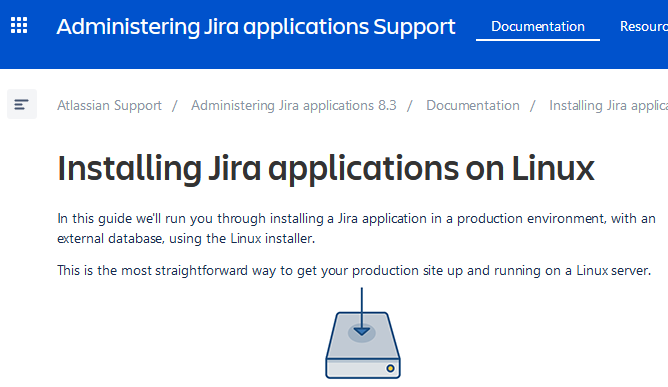
\includegraphics[width=1\textwidth]{resources/jira_installation}\\
		\caption{The issues related with Jira and Confluence are handled by a dedicated Jira Cloud instance}
	\end{figure}
	% todo aggiungere riferimento a paragrafo
	Jira needs a database in order to store all the information regarding projects, users, etc.
	For the first installation, which was made for testing purposes, the embedded H2 database was enough.
	%todo aggiungere a glossario h2 database 
	%todo aggiungere riferimento a documentazione
	%https://confluence.atlassian.com/jirakb/accessing-jira-s-h2-embedded-database-776818136.html
	It's important to note that the documentation says the H2 database is not suitable for production environments.
	
	%todo aggiungere immagine prima pagina di jira appena installato
	
	The first thing that I have done after the installation was getting acquainted with the interface and understanding how Jira's components interconnect with each other as I read in the documentation.
	To do this I have created some mock projects that I filled with issues; it's here that I understood the concept of Board in Jira.
	Experimenting with workflows was one of the most important things to do, because these are fundamental in an issue tracking system's configuration and are strictly connected to the concept of Board.
	
	% todo inserire immagine di board
	
	After understanding the fundamentals of this software and getting to know it's basic features, I went ahead and installed Portfolio.
	
	%todo aggiungere riferimento
	This plugin, as told in ... helps visualizing the issues on a roadmap, which was one of the most important requirements.
	%todo aggiungere riferimento a requisito
	
	Installing Portfolio was easy, I just followed the instructions on the documentation to install the latest version of the plugin.
	
	%todo inserire immagine di portfolio
	
	After installing Portfolio and creating plans for my mock up projects, I have chosen to install Service Desk, to complete the configuration of the Jira instance.
	As earlier I have followed the documentation on Jira's website.
	As described in ...aggiungere riferimento... this piece of software is used to communicate with the clients and having a portal from which a client can find information and request assistance with a product.
	The first thing I tested after installing this software was creating a portal and see from the point of view of a client how this can be able to open an issue and what type of issues he may have access to.
	
	%todo inserire immagine Service Desk
	
	Not long after I have installed Confluence, and like Jira, I have used it's embedded database.
	Both software run on the same system, and their services are offered on port 8080 and 8090 respectively for Jira and Confluence.
	Soon after I connected the software together and I tested it out by creating a knowledge base for a Service Desk project and a documentation space for a Software project.
	Confluence was easier to get familiar with, so after creating some mock spaces related to the projects that were in Jira at the time, I moved on.
	
	To facilitate the integration between these tools, Atlassian allows to have a single users table stored on either Jira or Confluence.
	So during, when during the installation of Confluence there an option to link it to Jira's instance was presented, I inserted the administrative credentials and told Confluence to use Jira's users.
	
	%todo aggiungere a glossario tomcat e webserver
	%todo aggiungere riferimento a http://tomcat.apache.org/
	Jira and Confluence both use an Apache Tomcat web server.
	To run them both on the same domain I had some issues regarding the login.
	Cookies for the users are stored for allowing them to access without inserting the password each time, but they didn't work correctly because the users were automatically logged out after some minutes.
	This was because, when running on the same domain, even if on different ports, cookies from Jira and Confluence go in conflict.
	%todo aggiungere riferimento
	%https://confluence.atlassian.com/jirakb/how-to-change-the-jira-application-context-path-225119408.html
	When looking on the Internet for answers I found that many people new to these software incur on the same situation.
	%todo inserire a glossario context path con riferimento da
	%https://www.eclipse.org/jetty/documentation/9.4.x/configuring-contexts.html
	To solve this issue all is necessary is to change the context path of the software's server.xml file that contains the configuration of the webserver.
	An example of changing the context path for this project is:
	\begin{center}
		\texttt{http://yourdomain.com:8080}
	\end{center}
	becomes:
	\begin{center}
		\texttt{http://yourdomain.com:8080/jira}
	\end{center}
	In case of Confluence, where the default port is 8090, the context path will be:
	\begin{center}
		\texttt{http://yourdomain.com:8090/confluence}
	\end{center}
	At this point there was a change in the requirements that were given to me by the tutor.
	Contrary to what he said, the IT department opted to use GitLab instead of BitBucket because the developers know it better and there is no billing for their usage tier.
	\hl{So it's free.}
	This meant that there would be ine less tool that needed to be installed, but I had to understand how to link Jira's functionalities to those offered by GitLab.
	Connecting these tools together means that a developer can interact with Jira's issues in a project by typing it's ID in the messages that he uses for commits, comments, merge requests and so on.
	Fortunately GitLab's documentation had a dedicated page with instruction examples and a guide that allowed me to configure both tools.
	%todo citare
	%https://docs.gitlab.com/ee/user/project/integrations/jira.html
	This functionality allows GitLab to interact with Jira's default workflows, which sometimes are too simple for some software projects.	
	Since the license for GitLab's hosted version is not Premium (or Silver for the online one) there is no interaction the other way around, from Jira to GitLab.
	%todo citare
	%https://docs.gitlab.com/ee/integration/jira_development_panel.html
	There is no 1:1 project mapping from GitLab to Jira, a commit message in the repository may reference multiple Jira issues from different projects.
	%todo aggiungere riferimento
	Later ... I will talk about installing a plugin that allows these tools to be better connected.
	After understanding the potentiality of this connection I went on and set up a small demo that touched all the things that I have covered in the first two weeks of the internship.
	Since my tutor wasn't available for a few days so I took the liberty to customize the environment by changing the colors and logos in the interface, putting Athonet's.
	
	% todo inserire immagine di interfaccia customizzata
	
	When he came back during the meeting I have taken with him, he said that he liked the work I have done and that it was time for more elaborate mock projects in order to present the tools' functionalities to other company figures.
	After that I have deleted the mock projects from Jira and the related spaces in Confluence to ask the IT department for a snapshot of the VM I was working on.
	
	This allowed me to have a baseline, a deliverable that I was able to use as a secure point in time in which I could go back if anything after went wrong.
	
\section{First realistic mock projects and feedback}
	
	The fourth week of the internship I was ready to implement more realistic projects in Jira, connecting them to Confluence providing them with documentation and creating a link with GitLab.
	The objective was to have a working demo that could be shown to various members of Athonet for them to understand how these software can be used in their departments.

	In Jira I have created the projects EPC and Dashboard, both Software projects, while in Confluence I have created the spaces EPC Documentation and Dashboard Documentation.
	Also in Jira I have created an Athonet Internal Wiki project, to show how Service Desk could be useful for sharing internal documents between employees.
	
	For the first project I have implemented a more articulate workflow that resembles the realistic evolution of an issue inside the company and customized the menus that allow the creation of an issue.
	Later these will be revised because in this stage I did not have the information about what an issue requires to have in Athonet's case. 
	
	As I continued working on the mock projects and creating issues, I noted down all the most important customization that an administrative user can use to set up the software, not only for Athonet's specific purposes but in general.
	
	To make the project more realistic I have created three user groups, besides the default ones, to which I have assigned three users each:
	\begin{itemize}
		\item Management
		\item Verification
		\item Developers
	\end{itemize}
	
	Every group had various permissions; that allowed me to demonstrate how basic security works in these tools.
	
	As I told the progress that I have made to the tutor, he was able to set a meeting with him, the verification manager and the developer manager.
	
	For this I prepared some slides to explain some of the nomenclature in Jira and the various things that I have implemented.
	
	The core of this meeting was a discussion between the managers that verted on understanding how the various projects could be implemented in such a way that the employees would not be forced to use a strict Agile methodology, but to accomodate them and let them understand how these tools work.
	
	This also meant that there would be a custom workflow that had to be implemented and the managers were happy to see that it could be easily done, as for customizing the issue creation and modification menu.
	
	
	They were also happy about the Internal wiki project because it meant that there could be one single tool for both internal documentation regarding clients and general notes for employees (like for example a guide on how to install Docker without loosing internet connectivity).
	
	After this meeting, I was put on standby because of the internal discussions that had to be done in order for the managers to understand how to adapt the workflow they had in Redmine for Jira and how to include Confluence in the mix.
	
	This was not considered when writing the plan of work document, but to carry on with the work I decided to start writing the documentation about installing and configuring the software, aimed for the administrators.
	
	In the sixth week, after this was done I showed it to the tutor and after his approval I started working on the user guide, which was written in the wiki Confluence space.
	This meant that in order for the users to understand how to use the tools, they had to start using the tools and search in them the "how to"s.
	
	Later on a new meeting was scheduled with the product owner, who wanted to understand better how Portfolio works and how the concept of product matches the project denomination in Jira.
	For him one of the most important things was to see how releases are mapped inside the software, since Redmine did not offer an intuitive interface and did not allow to see them on a timeline and applying filters.
	
	I showed him the progress I have made and he approved it, also he said that he wanted the credentials to start using it and see how to map the ongoing projects in Redmine to new ones in Jira or how to migrate them.
	
%	todo: spiegare che in questo periodo ho implementato un workflow che permette ad una issue di essere createa in service desk e che da li passa in business e che va in software, importante capire a quale release si riferisce
	
	The next week I had another meeting with more company figures: a senior developer, the business strategy manage, the managers that I have talked to in previous meetings, the CTO and my tutor.
	As in the other meetings I have explained the various software that I have installed, the purpose for each one of them and the evolution of an issue.
	
	Snapshot of the machine.
	
	--------------------------------------	--------------------------------------	--------------------------------------

\section{Transitioning to production}

	This phase corresponds to ... in the work plan

	After the approval for using the tools by other departments (R\&D) it's time to transition it / move it to production
	
	\subsection{Migrating data from Redmine}
		tool automatico di migrazione
		collegamento con redmine, lo fa in maniera automatica
		e se va male? c'è sempre lo snapshot
	
	\subsection{First non mock projects}
	
	\subsection{Fine tuning of the final product}
		interazione con le persone
		in base alle necessità degli utenti e di come lo usano faccio minime modifiche in produzione
		miglioramento della documentazione
	
	\subsection{How are these tools being used}
		è veramente agile? 
		è un dialetto?
		è un misto?
		perchè athonet lo sta usando in questo modo?

\section{Final feedback and what else could be implemented in the future}

	This phase corresponds to ... in the work plan

	\subsection{Final feedback from the users}
		feedback da parte del tutor
		
		feedback da responsabile strategia aziendale (gl)
		feedback da responsabile del prodotto (aka product ownner / hesham)
		feedback da responsabile sviluppo + testing
			
		feedback da parte di tutti gli utenti
	
	\subsection{What Athonet plans to do with these new tools}
		arrivare ad utilizzare agile in maniera rigida?
		continuare a fare misto?
